\documentclass[8pt]{beamer}\usepackage[]{graphicx}\usepackage[]{color}

\def\expect#1#2{\underset{#1}{\mathbb{E}}\left[#2\right]}
\def\sumn{\sum_{n=1}^N}
\def\x{x}
\def\xvec{X}
\def\w{w}
\def\onevec{1_N}
\def\infl{\psi}

\usetheme{metropolis}           % Use metropolis theme
\usepackage{amsmath}
\usepackage{tikz}
\usepackage{tikz}

\title{TikZ and Beamer for Image Annotation}
\author{Ryan Giordano}
\date{Nov 16th, 2021}
\institute{Massachusetts Institute of Technology}

\begin{document}



%%%%%%%%%%%%%%%%%%%%%%%%%%%%%%%%%%%%%%%%%%%%%%%%%%%%%%%%%%%%%%%%%%%%%%%
%%%%%%%%%%%%%%%%%%%%%%%%%%%%%%%%%%%%%%%%%%%%%%%%%%%%%%%%%%%%%%%%%%%%%%%
%%%%%%%%%%%%%%%%%%%%%%%%%%%%%%%%%%%%%%%%%%%%%%%%%%%%%%%%%%%%%%%%%%%%%%%

\begin{frame}{How does the IJ work?  Data re-weighting.}

Augment the problem with {\em data weights} $\w_1, \ldots, \w_N$.
%
We can write $\expect{p(\theta \vert \xvec, \w)}{\theta}$.

\begin{minipage}{0.49\textwidth}
    \hfill\\
    Let's annotate this.
\end{minipage}
\begin{minipage}{0.49\textwidth}
    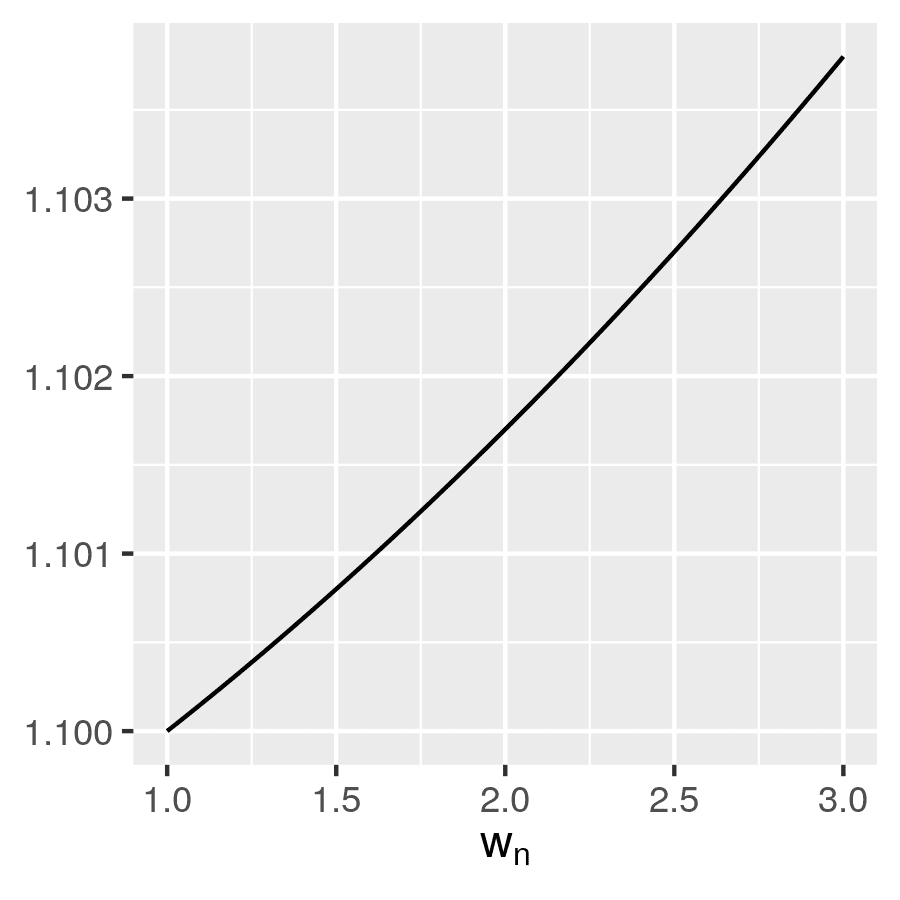
\includegraphics[width=0.98\textwidth]{e_beta_w}
\end{minipage}




\end{frame}







%%%%%%%%%%%%%%%%%%%%%%%%%%%%%%%%%%%%%%%%%%%%%%%%%%%%%%%%%%%%%%%%%%%%%%%
%%%%%%%%%%%%%%%%%%%%%%%%%%%%%%%%%%%%%%%%%%%%%%%%%%%%%%%%%%%%%%%%%%%%%%%
%%%%%%%%%%%%%%%%%%%%%%%%%%%%%%%%%%%%%%%%%%%%%%%%%%%%%%%%%%%%%%%%%%%%%%%

\begin{frame}{How does the IJ work?  Data re-weighting.}

Augment the problem with {\em data weights} $\w_1, \ldots, \w_N$.
%
We can write $\expect{p(\theta \vert \xvec, \w)}{\theta}$.

\begin{minipage}{0.49\textwidth}
    \hspace{\textwidth}
\end{minipage}
\begin{minipage}{0.49\textwidth}
    % https://www.overleaf.com/learn/latex/TikZ_package
    % https://latexdraw.com/how-to-annotate-an-image-in-latex/
    % https://tex.stackexchange.com/questions/9559/drawing-on-an-image-with-tikz
    \begin{tikzpicture}
        \onslide<6-> {
        \node[anchor=south west,inner sep=0] (image) at (0,0) {
            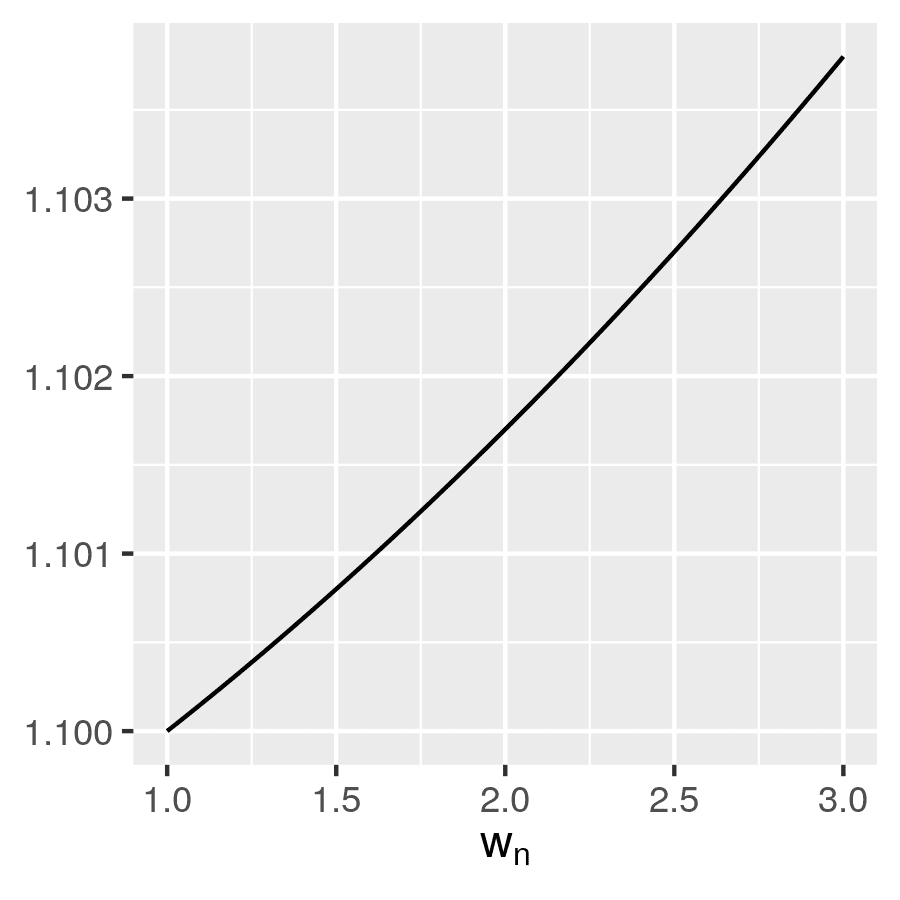
\includegraphics[width=0.98\textwidth]{e_beta_w}
        };
        }
        \onslide<7->{
        \begin{scope}[x={(image.south east)},y={(image.north west)}]
            \draw[blue, thick, <-] (0.2,0.23) -- ++(0.1,0.25)
                    node[above,black,fill=white]
                    {\small $\expect{p(\theta \vert \x)}{\theta}$};
        \end{scope}
        }
        \onslide<6->{
        \begin{scope}[x={(image.south east)},y={(image.north west)}]
            \draw[blue, thick, <-] (0.8,0.8) -- ++(-0.1,0.1)
                    node[left,black,fill=white]
                    {\small $\expect{p(\theta \vert \x, \w_n)}{\theta}$};
        \end{scope}
        }
        \onslide<9->{
        \begin{scope}[x={(image.south east)},y={(image.north west)}]
            \draw[red, thick, -] (0.18,0.18) -- ++(1.2 * 0.6, 1.2 * 0.48);
        \end{scope}
        }
        \onslide<10->{
        \begin{scope}[x={(image.south east)},y={(image.north west)}]
            \draw[blue, thick, <-] (0.8,0.65) -- ++(0.02,-0.1)
                    node[below,black,fill=white]
                    {\small Slope $ = \infl_n$};
        \end{scope}
        }
    \end{tikzpicture}
\end{minipage}


\end{frame}




\begin{frame}{Source and further reading}

Beamer:
{\tiny
% \url{https://www.overleaf.com/learn/latex/Beamer_Presentations%3A_A_Tutorial_for_Beginners_(Part_1)%E2%80%94Getting_Started}\\
\begin{itemize}
\item Google ``beamer tutorial''
\item \url{https://warwick.ac.uk/fac/sci/physics/research/cfsa/people/pastmembers/wuensch/workshoplatex/beamertutorialkwuensch.pdf}
\item \url{https://www.texdev.net/2014/01/17/the-beamer-slide-overlay-concept/}\\
\end{itemize}
}

TikZ:
{\tiny
\begin{itemize}
\item \url{https://www.overleaf.com/learn/latex/TikZ_package}
\item \url{https://www.math.uni-leipzig.de/~hellmund/LaTeX/pgf-tut.pdf}
\item \url{https://latexdraw.com/how-to-annotate-an-image-in-latex/}
\item \url{https://tex.stackexchange.com/questions/9559/drawing-on-an-image-with-tikz}
\end{itemize}
}

\end{frame}


\end{document}
